\selectlanguage{english}%

\chapter{Resultados}
\label{capRes}
A partir dos  
\section{Simulações} \label{secAnalise}
Foram realizadas simulações de resposta ao degrau do sistema de quatro-tanques modelado seguindo as abordagens apresentadas. Por se tratar de um problema multivariável com zeros alocáveis, simulou-se as respostas dos modelos para os casos de \textbf{fase-mínima} e de \textbf{fase não mínima}. Os resultados são observados nas seções a seguir.

\subsection{Fase Mínima}
A tabela a seguir apresenta as especificações do sistema, nota-se por $\gamma_1$ e $\gamma_2$ que o sistema está em fase mínima.

\begin{center}
	\begin{tabular}{|c|c|}
		\hline
		\multicolumn{2}{|c|}{Especificações Iniciais da Planta} \\
		\hline
		A1, A3 & 28 \\ \hline
		A2, A4 & 32 \\ \hline
		a1, a3 & 0.071 \\ \hline
		a2, a4 & 0.057 \\ \hline
		g & 981 \\ \hline
		k1 & 3,33 \\ \hline
		k2 & 3.35 \\ \hline
		$\gamma_1$ & 0.70 \\ \hline
		$\gamma_2$ & 0.60 \\ \hline
		\hline
	\end{tabular}
\end{center}

Realiza-se
\begin{figure}[H]
	\centering
	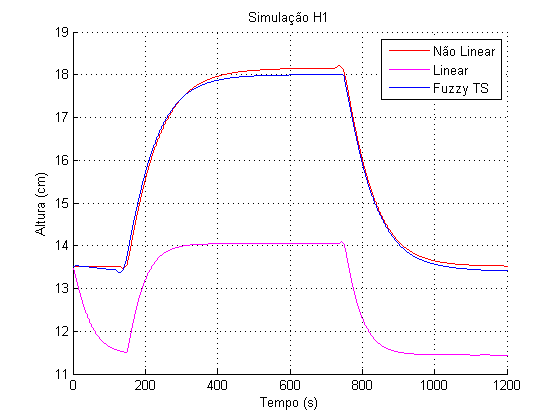
\includegraphics[width=0.7\textwidth]{img/FM_h1_5_10_15.png}
	\caption{\small Linearização Convencional: $ \bar{h1}=5, \bar{h2}=5$. Linearizações Fuzzy: $\bar{h1}=[10 \ \ 15] \ \ \bar{h2}=[10 \ \ 15]$ }
	\label{figH1FM_1}
\end{figure}

\begin{figure}[H]
	\centering
	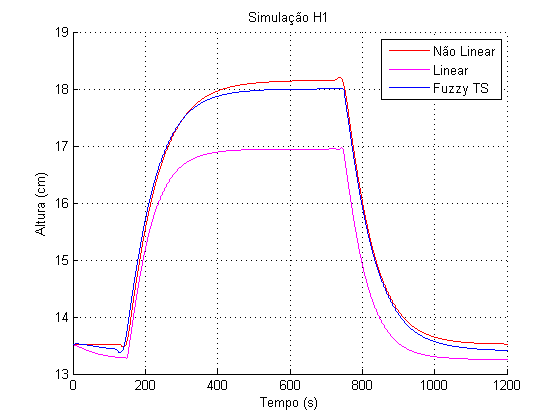
\includegraphics[width=0.7\textwidth]{img/FM_h1_10_15.png}
	\caption{\small Linearização Convencional: $ \bar{h1}=10, \bar{h2}=10$. Linearizações Fuzzy: $\bar{h1}=[10 \ \ 15] \ \ \bar{h2}=[10 \ \ 15]$ }
	\label{figH1FM_2}
\end{figure}

\begin{figure}[]
	\centering
	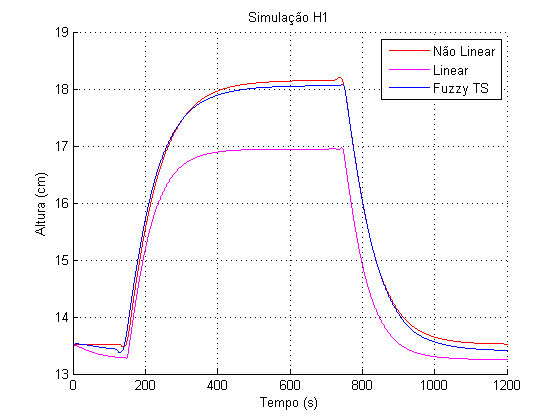
\includegraphics[width=0.7\textwidth]{img/FM_h1_10_15_20.png}
	\caption{\small Linearização Convencional: $ \bar{h1}=10, \bar{h2}=10$. Linearizações Fuzzy: $\bar{h1}=[10 \ \ 15 \ \ 20] \ \ \bar{h2}=[10 \ \ 15 \ \ 20]$ }
	\label{figH1FM_3}
\end{figure}

\subsection{Fase Não-Mínima}
A tabela a seguir apresenta as especificações do sistema, nota-se por $\gamma_1$ e $\gamma_2$ que o sistema está em fase não mínima.
\begin{center}
	\begin{tabular}{|c|c|}
		\hline
		\multicolumn{2}{|c|}{Especificações do sistema} \\
		\hline'
		A1, A3 & 28 \\ \hline
		A2, A4 & 32 \\ \hline
		a1, a3 & 0.071 \\ \hline
		a2, a4 & 0.057 \\ \hline
		g & 981 \\ \hline
		k1 & 3,14 \\ \hline
		k2 & 3.29 \\ \hline
		$\gamma_1$ & 0.43 \\ \hline
		$\gamma_2$ & 0.34 \\ \hline
		\hline
	\end{tabular}
\end{center}

Nas figuras que se seguem apresentam-se as respostas dos modelos à degraus aplicados ao sistema.  Observa-se que o modelo linear apresenta bons resultados quando o estado do sistema é próximo ao ponto de operação. Já para os modelos fuzzy, quanto mais pontos de linearização utilizados, melhor o resultado, embora mais complexo o custo computacional.

\begin{figure}[H]
	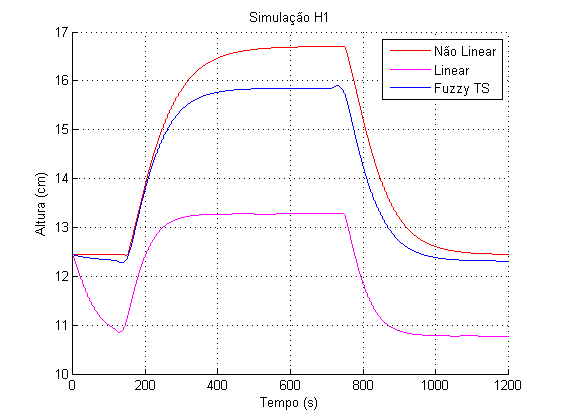
\includegraphics[width=0.5\textwidth]{img/h1Fuz5_10.png}
	\caption{\small Linearização Convencional: $ \bar{h1}=5, \bar{h2}=5$. Linearizações Fuzzy: $\bar{h1}=[5 \ \ 10] \ \ \bar{h2}=[5 \ \ 10]$ }
	\label{figH1FNM_1}
\end{figure}

\begin{figure}[H]
	\centering
	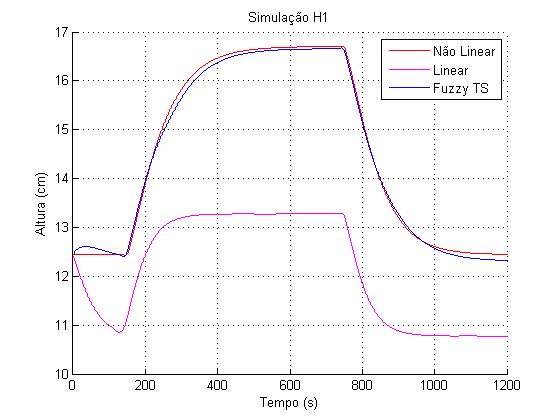
\includegraphics[width=0.7\textwidth]{img/h1Fuz5_10_15.png}
	\caption{\small Linearização Convencional: $ \bar{h1}=5, \bar{h2}=5$. Linearizações Fuzzy: $\bar{h1}=[5 \ \ 10 \ \ 15] \ \ \bar{h2}=[5 \ \ 10 \ \ 15]$ }
	\label{figH1FNM_2}
\end{figure}

\begin{figure}[H]
	\centering
	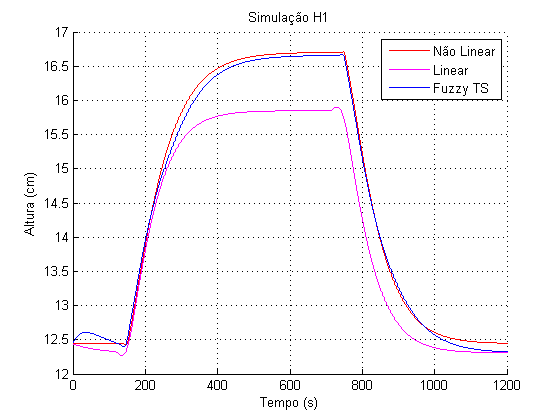
\includegraphics[width=0.7\textwidth]{img/h1conv10.png}
	\caption{\small Linearização Convencional: $ \bar{h1}=10, \bar{h2}=10$. Linearizações Fuzzy: $\bar{h1}=[5 \ \ 10 \ \ 15] \ \ \bar{h2}=[5 \ \ 10 \ \ 15]$ }
	\label{figH1FNM_3}
\end{figure}

\begin{figure}[H]
	\centering
	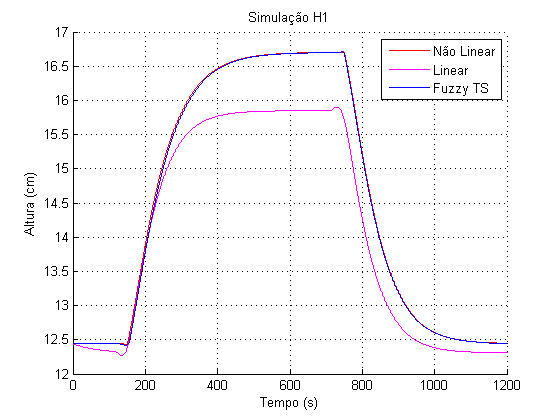
\includegraphics[width=0.7\textwidth]{img/h1Fuz_1to30.png}
	\caption{\small Linearização Convencional: $ \bar{h1}=10, \bar{h2}=10$. Linearizações Fuzzy: uma linearização a cada 1 centímetro para ambos os níveis.}
	\label{figH1FNM_4}
\end{figure}

Como explicado na seção anterior, o conjunto de regras é realizado a partir da combinação simples dos conjuntos de pontos das variáveis aferidas. Assim, na \hyperref[figH1FNM_4]{Figura \ref{figH1FNM_4}} haverão 900 regras, uma combinação de 30 pontos para $h_1$ e 30 pontos para $h_2$.


\section{Implementação}

\selectlanguage{brazil}%

